\documentclass[11pt]{article}
\usepackage{techreport}
\title{Landing on the Wrong Altimeter Setting:\texorpdfstring{\\}{} A Pre-registered Study of Business Jets and Airline Jets in Open ADS-B Data}
\shorttitle{Landing on the Wrong Altimeter Setting}
\author{James Le Cuirot\thanks{Commercial pilot (Senior First Officer), aviation flight safety officer, and aviation safety and compliance consultant specialising in human factors; MSc in Human Factors in Aviation.}\\[2pt] \normalsize CitadelAero}
\date{Working draft v0.4, 11 November 2026. Not peer reviewed}

\begin{document}
\setlength{\emergencystretch}{1.5em}
\maketitle

\begin{abstract}
An aircraft that lands with the wrong altimeter setting flies its barometric altitudes at the wrong height with no barometric indication of it. Two European studies have measured how often this happens; no published measurement was found for the United States, or one that compares types of operator. Modern aircraft broadcast the pressure setting selected on board. This study compared that broadcast setting with the consensus of other aircraft landing at the same airport within 30 minutes, at 119 US and European airports, in two pre-registered samples of 30 days in 2026 (about 714{,}000 and 730{,}000 landings). In the first sample business jets landed with a setting at least 2~hPa from the consensus more often than airline jets at the same airport on the same day (Mantel-Haenszel odds ratio 3.4). A second hypothesis, about Europe against the United States, was not supported, and review showed that the registered measure picked up a spurious switch to the standard setting in the final seconds on some European airliners. A corrected measure was then fixed in advance and tested on the second sample. The business-jet result replicated: odds ratio 4.0 (95\% interval 3.5 to 4.7; 2.7 to 5.4 when whole operators are resampled), and 13.9 (7.9 to 23.7) for errors of 5~hPa or more. In the second sample the setting was wrong by 2~hPa or more on 2.0 per 1{,}000 landings, by 5~hPa or more on 0.19, and by 10~hPa or more (about 280~ft) on 0.06. The consensus was within 1~hPa of the airport weather report for 97\% of landings, and the results were the same with the weather report as the reference. Nine in ten of the discrepancies are of 2 to 5~hPa and may not be errors in the operational sense. About half of the large errors recorded in Europe came from a few older aircraft that supply the value by a second route and show the standard setting on most landings; with those removed, errors of 5~hPa or more were two to three times as frequent in the United States as in Europe. Which altimeter the broadcast reflects is not defined, so on some business jets a wrong broadcast may not mean the crew flew on a wrong setting. Review of this draft has been by AI reviewers only.
\end{abstract}

\section{Introduction}\label{sec:intro}

On 23 May 2022 an Airbus A320 on a satellite-based approach to Paris-Charles de Gaulle descended to about six feet above the ground about 0.9~NM short of the runway. The controller had passed an altimeter setting 10~hPa too high, the crew set it, and every barometric indication on board looked normal~\cite{bea2024}. The European Union Aviation Safety Agency has issued and revised a safety bulletin on incorrect altimeter settings~\cite{easa2025}.

Two published measurements of how often aircraft land on a wrong setting were found, both in Europe. The French civil aviation safety directorate compared the setting downlinked to radar with the setting displayed to controllers for 1{,}694{,}266 landings at six French airports from 2019 to 2023. It found a difference of 2~hPa or more at the runway threshold on 2{,}269 landings (about 1.3 per 1{,}000) and of 10~hPa or more on 387 (about 0.23 per 1{,}000). About 27\% of the inconsistencies had the standard setting on board. The rate at Le Bourget, a business-aviation airport, was three times the rate at Charles de Gaulle, which the report attributed to ``very different fleets'' without further analysis~\cite{dsac2025}. A EUROCONTROL study built a detection algorithm on broadcast data and, as reported by France to an ICAO regional group, found 196 errors above 5~hPa in 747{,}353 flights at 378 European airports~\cite{mourousias2025,grepecas2026}. The full text of that paper could not be obtained for this study.

No published rate was found for the United States, and no study was found that compares business aviation with airlines or one region with another. The United States differs from Europe in two relevant ways. Settings are given in inches of mercury, and the change from the standard setting to the local one is made at 18{,}000~ft, well before the approach, where in Europe it is made at a few thousand feet~\cite{faaaim,dsac2025}.

This study uses open data to measure the rate at 119 airports in both regions and to test two pre-registered hypotheses: that business jets land on a wrong setting more often than airline jets at the same airport on the same day (H1), and that landing with the standard setting still selected is more frequent at European than at US airports (H2).

\section{Methods}\label{sec:methods}

The hypotheses, measures and analysis were committed to a public repository before any altimeter-setting data from the study days was read (branch \code{prereg/08-wrong-altimeter-setting}, commit \code{be41aa0}, 11 November 2026, 13:18 UTC). Section~\ref{sec:deviations} lists departures from that plan.

\paragraph{Data.} The adsb.lol archive publishes each day's ADS-B traces under an open licence~\cite{adsblol}. The study uses 30 UTC days in 2026, drawn at random for an earlier study of approach paths that never used the altimeter-setting field. Airports (119, chosen in advance, 76 in the United States and 43 in Europe) and aircraft types (65 business-jet and 58 airline jet types) were fixed lists. Airline-type aircraft were kept only with an airline-format callsign. Airport elevations came from OurAirports~\cite{ourairports}.

\paragraph{Setting at landing, as pre-registered.} A landing is the last airborne point of a track aligned with a runway and followed by ground movement or no later climb. The pre-registered setting at landing is the last value of the selected barometric pressure setting recorded for the aircraft in the 120~seconds before that point~\cite{readsb}. Values outside 940 to 1060~hPa were dropped.

\paragraph{Reference.} The reference for a landing is the median setting at landing of other aircraft landing at the same airport within 30~minutes either side. It required at least five other aircraft, at least 60\% of them within 1.0~hPa of their median. Landings without a reference were excluded.

\paragraph{Errors.} The difference is the setting at landing minus the reference. Thresholds were 2~hPa (primary), 5~hPa and 10~hPa. ``Standard left set'' means a setting within 0.5~hPa of 1013.25 that differed from the reference by 2~hPa or more. Two exclusions were made without regard to class: settings matching station pressure at airports above 300~ft (use of QFE), and all landings by any aircraft that was wrong on at least half of four or more landings.

\paragraph{Analysis.} H1: Mantel-Haenszel common odds ratio of an error of 2~hPa or more, business jet against airline jet, across strata of airport and UTC date, with a Cochran-Mantel-Haenszel test, a Robins-Breslow-Greenland interval and an interval from resampling whole airports. H2: the ratio of the rate of ``standard left set'' at European airports to that at US airports, among landings where the reference was at least 3~hPa from standard, with a $p$-value from permuting the region label across airports. Holm correction across the two tests. The method was built on one pilot day outside the sample, using pooled results and a run with shuffled labels; no result split by class or region was computed until all 30 days were processed.

\paragraph{Replication and weather-report check.} After the first sample was analysed and reviewed, a second pre-registration fixed the corrected measure of Section~\ref{sec:deviations} and four hypotheses (commit \code{7306d3b}, 11 November 2026, 14:39 UTC), and 30 further days were drawn at random from the 263 eligible days of 2026 not already used. Section~\ref{sec:replication} reports that study. It also compares the reference with the most recent routine or special weather report (METAR) at each airport issued in the 70 minutes before the landing, taken from the Iowa State University archive~\cite{iem}. That archive gives the setting in inches of mercury to two decimal places, so European values pass through a rounding of about 0.3~hPa. A third AI review of the replication led to the further post hoc analyses in Section~\ref{sec:third}.

\section{Deviations from the pre-registration}\label{sec:deviations}

The frozen code was run unchanged and its hashes match the pre-registration. Section~\ref{sec:registered} reports its results as registered.

\paragraph{A flaw in the registered measure, found in review.} Two independent AI reviewers (see Acknowledgement; all review of this paper has been by AI) found that the recorded field mixes two sources. One is the ADS-B broadcast at 0.8~hPa resolution; the other has 0.1~hPa resolution and is probably a Mode~S register decoded by the receiver software. On some aircraft, mostly European airliners, the second source shows the standard setting for a few seconds around touchdown after the correct setting had been shown throughout the approach. Because the registered measure takes the last value, it counted these as errors. They were about half of the European airline errors and most of the European ``standard left set'' events. A second problem was a small number of aircraft whose broadcast value jumped between impossible values.

\paragraph{Corrected measure (post hoc).} Section~\ref{sec:corrected} and everything after it use a corrected setting at landing: the most frequent value in the same 120-second window, with the landing excluded if three or more different values were recorded in the window. Everything else is as registered. Differences were rounded to 0.1~hPa before thresholds were applied. The corrected setting differed from the registered one on 1{,}784 landings, and 80 landings were excluded as unstable. All results on the corrected measure are post hoc.

\paragraph{Other.} The analyses in Sections~\ref{sec:posthoc} and \ref{sec:what} were designed after the results were seen. The two rate tables by aircraft type use lower cut-offs than the frozen script. Stratum dates span 31 UTC dates because three landings fell just after midnight.

\section{Results as pre-registered}\label{sec:registered}

\paragraph{Sample.} The 30 days held 809{,}959 landings: 714{,}916 by airline jets and 95{,}043 by business jets. A setting was recorded in the last two minutes on 97.0\% of them. After exclusions (27 implausible values, 3 landings on QFE, and 89 landings by 9 aircraft, 8 of them business jets, under the half-wrong rule), 713{,}835 landings were analysed: 650{,}307 by 17{,}617 airline aircraft and 63{,}528 by 11{,}618 business jets. Table~\ref{tab:coverage} shows that far fewer business-jet landings could be analysed.

\begin{table}[h]
\centering
\caption{Coverage by class and region.}\label{tab:coverage}
\begin{tabular}{lrrr}
\toprule
Group & Landings & Setting recorded & Analysed \\
\midrule
Airline jets, Europe & 275{,}237 & 99.6\% & 93.6\% \\
Airline jets, United States & 439{,}679 & 97.2\% & 89.3\% \\
Business jets, Europe & 17{,}416 & 97.9\% & 74.9\% \\
Business jets, United States & 77{,}627 & 86.9\% & 65.0\% \\
\bottomrule
\end{tabular}
\end{table}

\paragraph{H1.} Within the same airport and date, the odds ratio of an error of 2~hPa or more for business jets against airline jets was 3.42 (95\% interval 2.94 to 3.98; resampling airports, 2.77 to 4.27; Holm-adjusted $p < .001$; 684 informative strata). The crude rates over all airports were 8.53 per 1{,}000 (542 of 63{,}528) and 1.43 per 1{,}000 (930 of 650{,}307). H1 is supported.

\paragraph{H2.} Among eligible landings the standard setting was recorded on 71 of 188{,}811 in Europe (0.38 per 1{,}000) and 58 of 303{,}311 in the United States (0.19 per 1{,}000): rate ratio 1.97 (0.99 to 3.49; permutation $p = .072$). H2 is not supported.

\paragraph{Registered rates.} The registered measure gave 2.06 errors of 2~hPa or more per 1{,}000 landings, 0.26 of 5~hPa or more and 0.083 of 10~hPa or more. These are overstated in Europe for the reason given in Section~\ref{sec:deviations} and are superseded by Table~\ref{tab:rates}.

\section{Results on the corrected measure}\label{sec:corrected}

Nothing in this section is confirmatory. The European rates in it are overstated for a reason found later (Section~\ref{sec:third}).

\subsection{How often}

On the corrected measure 713{,}758 landings were analysed. The setting differed from the reference by 2~hPa or more on 1{,}411 (1.98 per 1{,}000; 95\% interval 1.80 to 2.17), by 5~hPa or more on 144 (0.20 per 1{,}000; 0.17 to 0.24), and by 10~hPa or more on 43 (0.060 per 1{,}000; 0.043 to 0.078). Table~\ref{tab:rates} and Figure~\ref{fig:rates} give the rates by region and class.

\begin{table}[h]
\centering
\caption{Landings per 1{,}000 with the setting wrong by at least the amount shown (corrected measure). Crude rates; event counts in brackets.}\label{tab:rates}
\begin{tabular}{lrrrr}
\toprule
 & Landings & 2 hPa & 5 hPa & 10 hPa \\
\midrule
Europe, all & 270{,}643 & 0.33 (89) & 0.16 (44) & 0.048 (13) \\
United States, all & 443{,}115 & 2.98 (1{,}322) & 0.23 (100) & 0.068 (30) \\
\midrule
Airline jets, Europe & 257{,}594 & 0.26 (67) & 0.10 (27) & 0.023 (6) \\
Airline jets, United States & 392{,}651 & 2.05 (804) & 0.14 (56) & 0.038 (15) \\
Business jets, Europe & 13{,}049 & 1.69 (22) & 1.30 (17) & 0.54 (7) \\
Business jets, United States & 50{,}464 & 10.27 (518) & 0.87 (44) & 0.30 (15) \\
\bottomrule
\end{tabular}
\end{table}

\begin{figure}[h]
\centering
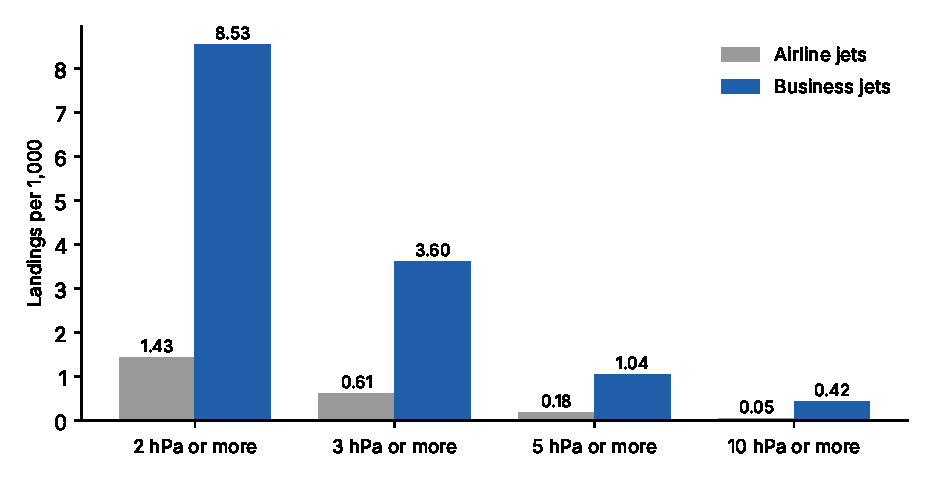
\includegraphics[width=0.85\textwidth]{figures/rates.pdf}
\caption{Landings per 1{,}000 with the setting wrong by at least the amount shown, corrected measure, crude rates.}\label{fig:rates}
\end{figure}

Three things stand out. Errors of 5~hPa or more were somewhat more frequent in the United States than in Europe (0.23 against 0.16 per 1{,}000). Errors of 2 to 5~hPa were about sixteen times as frequent in the United States (2.76 against 0.17 per 1{,}000). And the European rates are well below the two earlier European studies: 0.33 and 0.05 per 1{,}000 at 2 and 10~hPa against about 1.3 and 0.23 in the French study~\cite{dsac2025}, and 0.16 at 5~hPa against about 0.26 reported for EUROCONTROL~\cite{grepecas2026}. The French study used the radar downlink, which may be the same source that produced the spurious values removed here, but this was not tested.

\subsection{Business jets against airline jets}

On the corrected measure the H1 odds ratio was 3.46 (2.97 to 4.02; resampling airports, 2.81 to 4.29). It held under the pre-registered sensitivity analyses re-run on the registered measure, which gave between 3.1 and 5.1: excluding periods of changing pressure (4.0), a 15-minute reference window (3.5), aircraft with three or more landings (3.1), the United States alone (3.3), Europe alone (5.1; 2.9 to 9.0), adding the hour to the strata (3.6), ground-confirmed landings only (3.2), and leaving out each airport in turn (3.3 to 3.7). The reviewers confirmed it with conditional and fixed-effects logistic models (3.4 to 3.5), with the reference built from airline aircraft only (3.7), and at airport-dates where at least 90\% of landings of both classes could be analysed (3.7).

\paragraph{By size of error.} For errors of 2 to 5~hPa the odds ratio was 3.1 (2.7 to 3.7), on 293 business-jet and 777 airline events in informative strata. For 5~hPa or more it was 8.6 (5.2 to 14.2), on 49 and 79 events. For 10~hPa or more it was 16.8 (6.9 to 41.2), on 21 and 20 events. The larger ratios are imprecise, and the strata that inform them differ from threshold to threshold, so they should not be read as a smooth trend.

\paragraph{By how often the aircraft was seen.} The gap narrows among aircraft that landed often in the sample (Table~\ref{tab:util}). Restricted to aircraft with ten or more landings the odds ratio was 2.6 (2.1 to 3.1), and with twenty or more, 2.0 (1.4 to 2.8). Of the 22 business-jet errors of 10~hPa or more, 19 were by aircraft with fewer than ten landings in the sample. Counting one randomly chosen landing per aircraft gave a median odds ratio of 2.7 over 30 draws (range 2.1 to 4.2).

\begin{table}[h]
\centering
\caption{Errors of 2~hPa or more per 1{,}000 landings, by the number of landings the aircraft made in the sample.}\label{tab:util}
\begin{tabular}{lrrrrr}
\toprule
Landings by the aircraft & 1 & 2--3 & 4--9 & 10--19 & 20 or more \\
\midrule
Business jets & 13.5 & 10.8 & 10.4 & 7.2 & 5.2 \\
Airline jets & 16.4 & 3.0 & 1.5 & 1.5 & 1.3 \\
\bottomrule
\end{tabular}
\end{table}

\paragraph{By airport.} The crude business-jet rate rose with the share of business jets at the airport: 3.0 per 1{,}000 where they were under 5\% of traffic, 5.8 at 5 to 20\%, 8.5 at 20 to 60\% and 18.3 above 60\%. Airline rates rose too (1.1, 1.4, 2.7 and 7.6). At business-aviation airports the reference is mostly made of other business jets and is noisier, so the pooled crude rate of 8.5 per 1{,}000 overstates what a like-for-like comparison shows. Requiring a reference from ten or more aircraft with over 95\% agreement gave an odds ratio of 4.9 (3.9 to 6.1).

\paragraph{By operator and type.} Among the 60 airline callsign groups with at least 1{,}500 landings, rates ran from 0 to 14 per 1{,}000 with a median of 0.5; several large carriers had none. Regional jets were highest among airline types (2.6 to 5.1 per 1{,}000). Business-jet types with at least 1{,}000 landings ran from 3.1 to 16.2 per 1{,}000. The spread between operators is as wide as the gap between the classes.

\subsection{Standard setting at landing}

On the corrected measure H2 gave a rate ratio of 0.95 (0.52 to 1.60; $p = .85$). The apparent European excess in Section~\ref{sec:registered} was the artefact.

The registered definition also catches ordinary small differences that happen to fall on 1013. Requiring the setting to be at 1013 and at least 5~hPa from the reference leaves 53 landings (Table~\ref{tab:std}). These were about half of business-jet errors of 5~hPa or more (32 of 61) and a quarter of airline ones (21 of 83). Within the same airport and date, business jets had far higher odds (32; 13 to 77), on 27 and 19 events.

\begin{table}[h]
\centering
\caption{Landings with 1013 selected and the reference at least 5~hPa away.}\label{tab:std}
\begin{tabular}{lrrr}
\toprule
Group & Eligible landings & Events & Per 1{,}000 \\
\midrule
Airline jets, Europe & 158{,}123 & 15 & 0.095 \\
Airline jets, United States & 218{,}843 & 6 & 0.027 \\
Business jets, Europe & 8{,}040 & 14 & 1.74 \\
Business jets, United States & 27{,}437 & 18 & 0.66 \\
\bottomrule
\end{tabular}
\end{table}

\subsection{Other observations}\label{sec:posthoc}

\begin{itemize}
\item \textbf{Small errors in the United States.} Of US errors, 74\% for airline jets and 86\% for business jets had been held unchanged for five minutes or more. Airline small errors bunched in the first ten minutes of each hour (177, against 101 to 127 in the other ten-minute periods), which fits the hourly weather update. Business-jet small errors were flat across the hour (74 to 87).
\item \textbf{Direction.} Errors of 2~hPa or more were evenly split. Of errors of 5~hPa or more, 50 were set too high, which puts the aircraft lower than indicated, and 94 too low.
\item \textbf{Pressure far from standard.} On the registered measure, errors of 10~hPa or more rose with distance of the local setting from standard: for airline jets 0.007, 0.05 and 0.24 per 1{,}000 within 5~hPa, 5 to 15~hPa and beyond 15~hPa; for business jets 0.21, 0.46 and 1.35.
\item \textbf{Repeat errors.} Errors were rarely repeated by the same aircraft. A reviewer found that 533 of the 542 business-jet errors came from aircraft that broadcast different values on other flights, and that 530 held one steady value through the approach.
\item \textbf{Paris.} Le Bourget had too few analysable landings (873) to test the French threefold difference.
\end{itemize}

\section{Replication on a second sample}\label{sec:replication}

The four hypothesis tests in this section are confirmatory. The measure, exclusions, hypotheses and code were fixed before any of the second sample was downloaded, and the frozen script was run once after all 30 days were processed. The rates, secondary analyses and weather-report check were planned in advance but are descriptive.

\paragraph{Sample.} One drawn day (27 March) could not be processed and was replaced by the first reserve day (25 March), as the plan provided; one trace file on the reserve day could not be read. The 30 days held 825{,}926 landings. No setting was recorded on 24{,}198; 74 were unstable (three or more values in the window), 20 had implausible values, 3 matched QFE, and 53 were by 6 aircraft, all business jets, excluded under the half-wrong rule. With landings lacking a reference also removed, 730{,}324 were analysed: 667{,}394 by airline jets and 62{,}930 by business jets. Coverage matched the first sample (analysed: airline jets 93.9\% in Europe and 89.3\% in the United States; business jets 75.1\% and 65.7\%). Strata span 33 UTC dates because three landings fell just after midnight. The days are new but the aircraft mostly are not: 99.9\% of airline and 96.6\% of business-jet landings were by aircraft that also appear in the first sample.

\paragraph{Hypotheses.} All four were supported after Holm correction (Table~\ref{tab:rep}). The primary hypothesis also met its pre-set replication criterion, an odds ratio between 2 and 6. The registered interval from resampling whole airports was 3.2 to 5.3 for R1 and 9.4 to 21.4 for R2.

\begin{table}[h]
\centering
\caption{Business jets against airline jets within airport and date. Mantel-Haenszel odds ratios; business-jet and airline events in informative strata in square brackets. The first interval is the registered Robins-Breslow-Greenland one. The second, for the second sample, comes from resampling whole operators (post hoc) and is the one to rely on. First-sample figures are post hoc on the corrected measure.}\label{tab:rep}
\footnotesize\setlength{\tabcolsep}{4pt}
\begin{tabular}{lll}
\toprule
Outcome & First sample & Second sample \\
\midrule
R1: wrong by 2 hPa or more & 3.5 (3.0--4.0) [342, 856] & 4.0 (3.5--4.7; 2.7--5.4) [377, 877] \\
R2: wrong by 5 hPa or more & 8.6 (5.2--14.2) [49, 79] & 13.9 (8.9--21.8; 7.9--23.7) [64, 63] \\
R3: as R1, aircraft with 10+ landings & 2.6 (2.1--3.1) [130, 797] & 2.6 (2.1--3.2; 1.7--3.6) [135, 830] \\
R4: 1013 at landing, 5 hPa+ away & 32 (13--77) [27, 19] & 35 (16--78; 12--114) [34, 18] \\
\bottomrule
\end{tabular}
\end{table}

\paragraph{Rates.} The setting was wrong by 2~hPa or more on 2.04 per 1{,}000 landings (1.85 to 2.25), by 5~hPa or more on 0.19 (0.16 to 0.23) and by 10~hPa or more on 0.060 (0.043 to 0.079), against 1.98, 0.20 and 0.060 in the first sample. Table~\ref{tab:rates2} gives the rates by group.

\paragraph{Secondary analyses.} The odds ratio was 3.4 (2.9 to 4.0) for errors of 2 to 5~hPa and 20 (9 to 44) for 10~hPa or more, on 19 and 21 events. It was 3.9 in the United States and 7.4 (4.3 to 13.0) in Europe, 3.8 with the hour added to the strata, 4.8 with the strict reference, and 3.1 among aircraft with four or more landings. Among aircraft with twenty or more landings it was 2.2 (1.6 to 3.0). The pattern in Table~\ref{tab:util} recurred: business-jet rates fell from 19.9 per 1{,}000 for aircraft seen once to 6.4 for those seen twenty times or more, against 1.3 for airline aircraft seen that often.

\paragraph{The reference against weather reports.} The consensus reference was within 1.0~hPa of the latest weather report for 97.5\% of 724{,}718 landings (97.2\% in Europe, 97.6\% in the United States) and within 1.7~hPa for 99.9\%. The first sample gave 97.4\% and 99.9\% (post hoc). Agreement was lower at airports where business jets were over 60\% of traffic (94.3\%), and Palm Beach was missing from the weather data. The consensus therefore tracks the published setting.

The frozen script also used the weather report as the reference in place of the consensus, which brings in about 17{,}000 business-jet landings that had too little other traffic for a consensus. As run, it gave odds ratios of 2.8 (2.5 to 3.1) at 2~hPa and 9.4 (6.6 to 13.4) at 5~hPa. The third review showed that neither figure is comparable with Table~\ref{tab:rep}, for two reasons. First, the archive contains a few corrupt reports (25 found, such as 40.00~inHg at London Heathrow), and every airline landing that follows one is counted as a large error; with those reports removed the 5~hPa odds ratio is 13.1 (8.9 to 19.3). Second, the broadcast moves in steps of 0.8~hPa, so against a consensus of other broadcasts a threshold of 2~hPa is in effect 2.4~hPa, while against a weather report it also admits differences of two steps. At a matched threshold of 2.4~hPa the weather-referenced odds ratio is 4.0 (3.4 to 4.7). With both corrections, which are post hoc, the two references give the same answer. The first sample gives 3.5 at 2.4~hPa and 11.5 at 5~hPa.

\paragraph{A labelling error in the frozen script.} In the output of the United States against Europe comparison the two rate labels are transposed. The ratio and $p$-value are unaffected.

\section{Checks made after review of the replication}\label{sec:third}

Everything in this section is post hoc. Results are in \code{results/after\_review3\_sample1.json} and \code{after\_review3\_sample2.json}.

\paragraph{A second-source artefact remains in Europe.} The ADS-B broadcast carries the setting in steps of 0.8~hPa. A value that is not on that grid can only have come from the second, 0.1~hPa source described in Section~\ref{sec:deviations}. Such landings were 562 of 277{,}801 analysed European landings in the second sample (0.2\%) and 8 in the United States, but they were 23 of the 44 European errors of 5~hPa or more (17 of 44 in the first sample). The reviewer traced them to a small number of older aircraft, among them A300-600 freighters and 737 Classics, that show a value at or near 1013 on most or all of their landings and made too few landings to trip the half-wrong rule. These are far more likely to be an avionics or decoding property than crews landing on the standard setting. Table~\ref{tab:rates2} therefore gives rates for all landings and for landings with a value on the broadcast grid. The grid test is approximate, since one 0.1~hPa value in eight falls on the grid by chance.

\begin{table}[h]
\centering
\caption{Second sample: landings per 1{,}000 with the setting wrong by at least the amount shown. Crude rates. ``Grid'' rows keep only values on the 0.8~hPa broadcast grid (post hoc).}\label{tab:rates2}
\begin{tabular}{lrrrr}
\toprule
 & Landings & 2 hPa & 5 hPa & 10 hPa \\
\midrule
Airline jets, Europe & 265{,}161 & 0.31 & 0.11 & 0.041 \\
\quad grid only & 264{,}679 & 0.21 & 0.045 & 0.015 \\
Airline jets, United States & 402{,}233 & 2.03 & 0.10 & 0.030 \\
Business jets, Europe & 12{,}640 & 1.98 & 1.19 & 0.47 \\
\quad grid only & 12{,}560 & 1.51 & 0.72 & 0.40 \\
Business jets, United States & 50{,}290 & 11.3 & 1.07 & 0.30 \\
\midrule
All landings & 730{,}324 & 2.04 & 0.19 & 0.060 \\
\quad grid only & 729{,}754 & 2.00 & 0.16 & 0.049 \\
\bottomrule
\end{tabular}
\end{table}

The business-jet comparison is not affected: on grid values only, R1 is 4.0 (3.4 to 4.6), R2 14.4 (8.9 to 23.5) and R3 2.6. R4 becomes 74 (21 to 257), on 28 business-jet and 7 airline events; 16 of the 18 European airline ``1013 at landing'' events in the second sample were off the grid. The first sample gives 3.4, 7.3 and 33.

\paragraph{The United States against Europe.} On all landings, errors of 5~hPa or more were 1.3 times as frequent in the United States (0.21 against 0.16 per 1{,}000; permutation $p = .22$). On grid values only they were 2.8 times as frequent (0.21 against 0.076; resampling airports, 1.7 to 5.3; $p < .001$), and 2.2 times in the first sample ($p = .002$). The difference is not adjusted for the mix of traffic.

\paragraph{Dependence between landings.} Two fractional-ownership operators flew 26\% of the analysed business-jet landings. Resampling whole operators (airline callsign prefix; business jets without one treated singly) widens the R1 interval to 2.7 to 5.4, and resampling airports gives 3.1 to 5.4, against 3.5 to 4.7 for the registered interval. Table~\ref{tab:rep} gives the operator-level intervals. The reviewer also found that business jets with an error in the first sample had a higher rate in the second (14.3 against 8.5 per 1{,}000), so the two samples are not independent at the level of the aircraft.

\paragraph{Implausible large values.} Five of the 21 business-jet errors of 10~hPa or more in the second sample, and five of 22 in the first, were non-standard values 30~hPa or more from the reference, against none and one for airline jets. The reviewer inspected the traces and judged four in the second sample to be corrupt broadcasts and one a plausible one-inch slip. Excluding all of them, R2 is 13.0 (8.2 to 20.5) and the 10~hPa odds ratio 15.8 (7.0 to 35.9).

\paragraph{1013 at landing on business jets.} The reviewer examined the traces of all 35 such business-jet landings in the second sample. On 28 the value was 1013 throughout the observed part of the approach, which was the last four to ten minutes; five showed a change to 1013 during it. All were one-off for the aircraft. They are not stuck transponders and not the touchdown artefact, but the traces cannot show whether the crew's own altimeter was also at 1013.

\section{What the result does and does not show}\label{sec:what}

\paragraph{What is established.} Compared at the same airport on the same day, the odds that a business jet lands with a broadcast altimeter setting 2~hPa or more from that of other aircraft are about three and a half to four times those for an airline jet. Crude rates differ more, about 9 against 1.3 per 1{,}000 landings, because business jets land more at airports where rates are higher for everyone. The result was confirmed in a second pre-registered sample of new days and is the same when the airport weather report is the reference. With allowance for landings by the same operator the interval is about 2.7 to 5.4. It survives correction of the measure, every sensitivity analysis, alternative statistical models, an airline-only reference, and restriction to well-covered airports. It is not produced by a few faulty transponders.

\paragraph{Most of it is small.} Nine in ten of the discrepancies behind that result are between 2 and 5~hPa, mostly 2.4 or 3.2~hPa, equivalent to about 65 to 90~ft. What they are is not established. In the first sample, airline small discrepancies in the United States bunched just after the hourly weather update, which points to settings not yet renewed, and business-jet ones did not. But in the second sample only 24\% of airline and 11\% of business-jet small discrepancies in the United States matched a setting published for the destination in the previous two hours. A setting taken from another station is one possible explanation and was not tested; a setting from a station within 100~NM is legitimate en route. These are best described as discrepancies from the local setting, not errors in the sense of the Paris incident.

\paragraph{The large errors are few.} Errors of 5~hPa or more occurred on about 1 business-jet landing per 1{,}000 against about 0.13 for airline jets. The second sample gave the same rates. The ratio is large and was confirmed, and it is the safety-relevant finding. In each sample it rests on 60 to 70 business-jet events, about half of them with 1013 selected. At 10~hPa most came from aircraft seen fewer than ten times (19 of 22 and 15 of 21), and about a quarter look like corrupt values.

\paragraph{The broadcast may not be the altimeter the crew flew on.} The standards define the field as the setting selected by the crew but not which side it comes from~\cite{eurocontrol2024}. An AI reviewer asked to take an avionics perspective noted that on some light jets flown by one pilot, the transponder may take its setting from the unused side, and that such aircraft often lack a warning when the two sides disagree. The data cannot exclude that reading. In the first sample 1013 at landing appeared commonest in older and lighter types, but in the second it occurred across 22 types, including recent ones with integrated flight decks, so the type pattern gives it no clear support either. On this reading some business-jet ``standard at landing'' events are an unset second altimeter and not a crew flying on the wrong setting. That would still mean no cross-check between the two sides was made.

\paragraph{The United States against Europe.} Once the second-source values are set aside, errors of 5~hPa or more were two to three times as frequent in the United States as in Europe, in both samples. This does not support treating the problem as a European one that the 18{,}000~ft transition altitude prevents. The comparison is post hoc and crude: it does not adjust for the mix of traffic, and the European rates here are well below both earlier studies, which may have included the same second-source values.

\paragraph{Consequences.} A 10~hPa error is about 280~ft. On an approach with ground-based vertical guidance the glidepath is unaffected, but the decision altitude, the altitude check on the glidepath, step-down and missed-approach altitudes are all displaced. On an approach using barometric vertical guidance the whole path is displaced~\cite{bea2024}. Radio altimeters, terrain warning using satellite height and controller warnings remain as defences. The study does not know which type of approach was flown.

\section{Limitations}\label{sec:limitations}

\begin{itemize}
\item \textbf{The measure is not direct.} The recorded value combines two sources that can disagree, and which altimeter either reflects is unknown. Values from the second source could be separated only approximately. The corrected measure was chosen after seeing the problem in the first sample, then fixed in advance for the second.
\item \textbf{Review.} The paper has been reviewed only by AI reviewers. Some figures attributed to ``the reviewer'' were not re-derived by the author's analysis; \code{AUDIT.md} lists which. The pre-registrations, analysis and review all took place on one day, and the commit times are not independently certified.
\item \textbf{Inferred reference.} The reference is the consensus of other aircraft. A wrong value given to every aircraft would not be detected. It agreed with weather reports within 1~hPa for 97\% of landings; Palm Beach was missing from the weather data.
\item \textbf{Coverage and selection.} Only 65\% of US and 75\% of European business-jet landings could be analysed, against about 90\% for airline jets. The missing landings are aircraft that do not broadcast a setting, which is optional in the United States, and landings with too little other traffic. A reviewer found that business-jet types with lower broadcast coverage had higher error rates among the aircraft that did broadcast, so the direction of any bias is unknown. Measured against weather reports, landings without a consensus reference had higher discrepancy rates in both classes (business jets 9.6 against 7.4 per 1{,}000, airline jets 2.4 against 0.9, second sample), so the published rates are probably too low.
\item \textbf{Exposure.} Airline aircraft averaged 37 landings in the sample and business jets 5.5. The per-landing comparison is dominated by rarely seen business jets, and the gap is smaller among frequently seen aircraft.
\item \textbf{Lag counted as error.} A crew holding a correct but older value is counted at the 2~hPa threshold.
\item \textbf{Resolution.} The broadcast has 0.8~hPa steps, so 2~hPa is effectively 2.4~hPa except where the reference falls on a half step.
\item \textbf{Classes.} The airline class includes cargo and some military and government flights with airline-format callsigns. Operator type is inferred from aircraft type and callsign. Test and training flights are included.
\item \textbf{No operational context.} Approach type, weather, minima, crew composition and what ATC said are unknown.
\item \textbf{Sample.} Sixty days in 2026 at 119 airports chosen by judgement. The second sample has new days but the same airports and almost entirely the same aircraft, so it confirms that the result is stable over time and was not produced by choices made after seeing the data. It does not show that the result would hold for other airports or fleets.
\item \textbf{Prior work not fully read.} The EUROCONTROL paper was seen only as an abstract and through secondary reports, and its figures quoted here come from a secondary source. It may contain breakdowns that this paper describes as not found. No systematic search was made for unpublished monitoring by air navigation service providers.
\end{itemize}

\section*{Acknowledgement}
\paragraph{AI assistance.} Literature searches, drafting and source verification were carried out with AI assistance (Claude, Anthropic) under the author's direction, as were the code and analysis. Three independent AI reviewers (two on the first sample, one on the replication), which had not seen the work being produced, checked the analysis and the claims against the data; their findings changed the paper and are recorded in \code{AUDIT.md}. The author is responsible for the final text.
\paragraph{Competing interests.} The author is the founder of CitadelAero, which builds AI tools for aviation, and is employed as a business-jet pilot.
\paragraph{Disclaimer.} The views expressed are the author's own and do not represent those of any employer or regulator. Nothing here is operational, legal or regulatory advice.
\paragraph{Materials.} The pre-registration, code, results and audit record for this paper are at \url{https://github.com/JamesLeCuirot/Research/tree/prereg/08-wrong-altimeter-setting/papers/08-wrong-altimeter-setting}.

\bibliographystyle{IEEEtran}
\bibliography{references}
\end{document}
